\section{Results}
\label{sec:results}
In this section, we analyze the quantitative and 
qualitative data collected during the quiz and interview phases 
to address the research questions in Section~\ref{sec:study_design}. 
We first discuss the results of the quiz phase tasks. 
We then present participants’ experiences in using \noah and Excel 
based on the interview and survey responses.

\subsection{Analysis of the Quiz Phase}
We first compare the participants’ task completion time 
and accuracy for \noah with Excel.  
\begin{figure}[t]
   \centering
\begin{tabular}{c c}  %trim=left bottom right top
 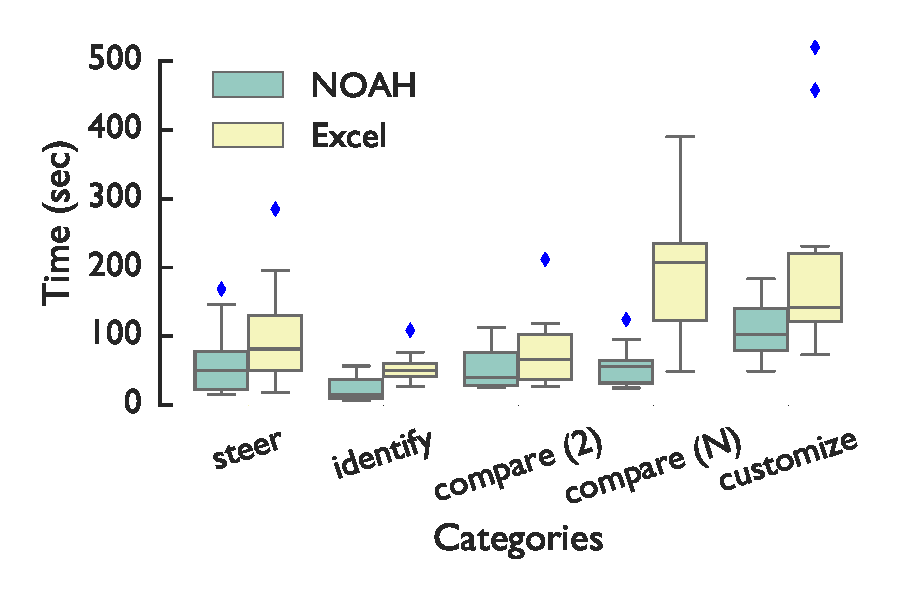
\includegraphics[width=0.23\textwidth,trim={18 20 20 15},clip]{images/bird_box.pdf} &
   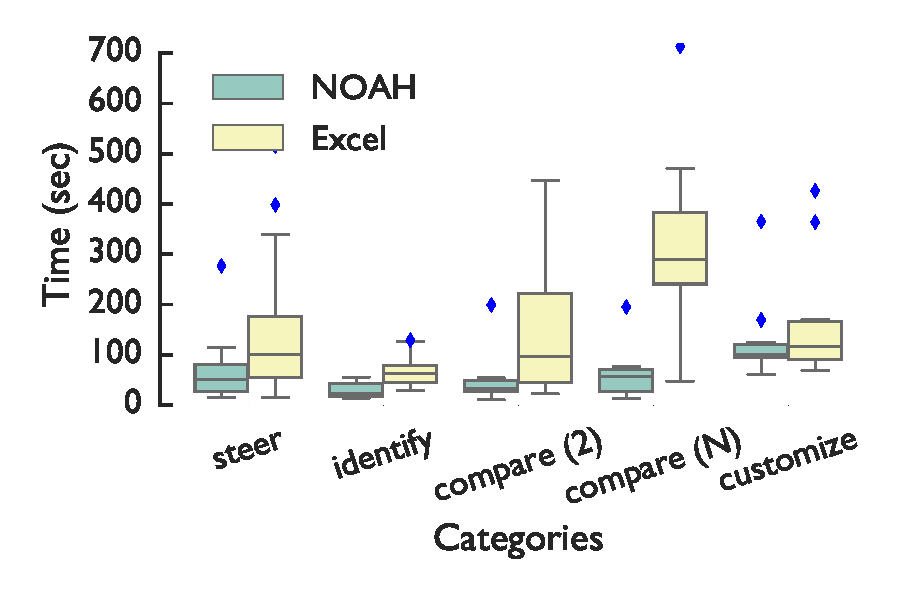
\includegraphics[width=0.23\textwidth,trim={18 20 20 15},clip]{images/airbnb_box.pdf} \\
   \textbf{(a) birdstrikes} & \textbf{(b) airbnb} \\
\end{tabular}
\vspace{-13pt}
\caption{Submission times per category for each dataset. Median submission times are much smaller for \noah compared to Excel.}
\vspace{-20pt} 
\label{fig:timeBox}
\end{figure}

\subsubsection{Comparison of Task Completion Time and Accuracy (\emph{RQ1})}
\stitle{Distribution of Completion Times.}
In Figure~\ref{fig:timeBox}a and~\ref{fig:timeBox}b, 
we show the distribution of submission times of participants 
for the four task categories, for birdstrikes and airbnb respectively. 
For most categories, 
\emph{participants’ median submission time for \noah 
was less than the fastest submission time for Excel},
confirming that the new capabilities offered by \noah
makes spreadsheet navigation faster. 

\stitle{Accuracy Distribution.} In Figure~\ref{fig:acc}a and~\ref{fig:acc}b, 
we show the percentage of correct submissions for the four task categories, 
for birdstrikes and airbnb respectively. 
For all the tasks except for \cmpA---for which the accuracy
was the same for both tools---participants 
attained slightly higher accuracy
with \noah compared to Excel. 
\toappendix{Analysis of screen capture for \cmpA 
revealed that between Florida---the correct answer---and California, 
three participants ($P12$, $P13$, and $P20$) out of 20 
chose the latter when using \noah.}

Since we conducted the study 
on a small population (20), 
we further evaluated the statistical significance of the results---see our supplementary material.
For all tasks except customize, the difference in completion times was statistically significant. 
However, the difference in accuracies was statistically significant 
for the steer tasks only. 

\begin{figure}[!htbt]
\vspace{-7pt}
   \centering
\begin{tabular}{c c} %trim=left bottom right top
   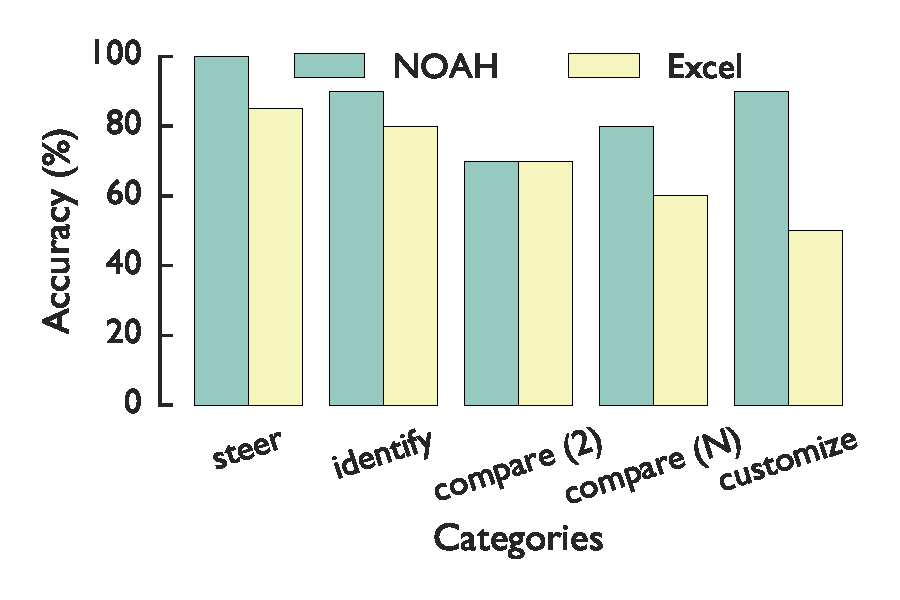
\includegraphics[width=0.23\textwidth,trim={18 20 20 20},clip]{images/bird_accC.pdf} &
   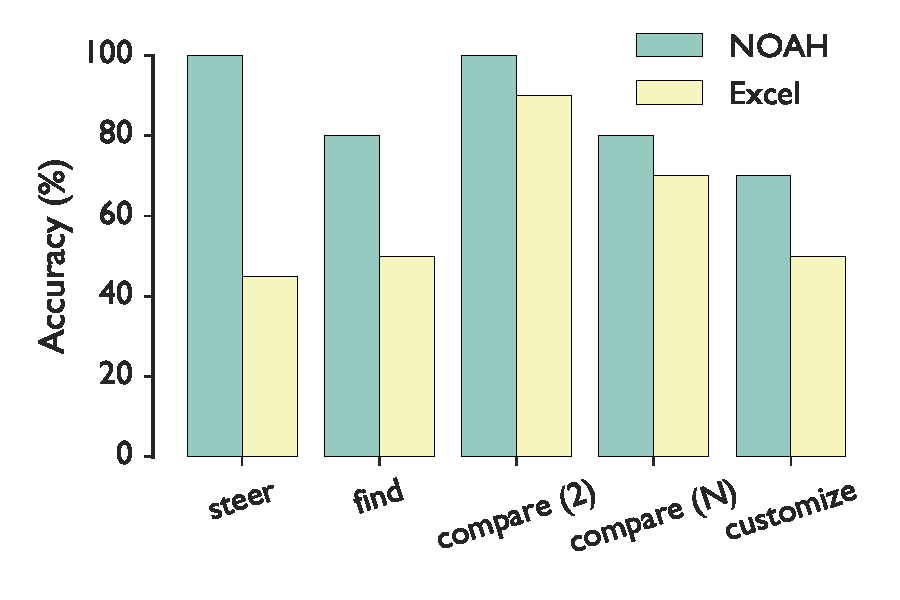
\includegraphics[width=0.23\textwidth,trim={18 20 20 20},clip]{images/airbnb_accC.pdf} \\
   \textbf{(a) birdstrikes} & \textbf{(b) airbnb} \\
\end{tabular}
\vspace{-13pt}
\caption{Per category accuracy for each dataset. Participants attained higher accuracy while completing tasks in NOAH compared to Excel.}
\vspace{-10pt}   
\label{fig:acc}
\end{figure}
\toappendix{
\stitle{Statistical Significance Testing.} Since we conducted the study on a small population (20 participants), we further evaluated the statistical significance of the results explained earlier. To measure the significance of the task completion times, we ran \emph{Mann-Whitney's U test} (as completion times did not follow a normal distribution). \emph{For all of the tasks except the customize task, we found a significant effect of the tools, \ie the response times for the tasks significantly differed by the choice of the tool} (see Table~\ref{tab:statTest}). On the other hand, we ran the \emph{Fisher's exact test} that measures statistical significance of categorical data (0/1 accuracy): \emph{only for steer tasks, the percentage of the accuracy of submissions significantly differed by the choice of the tool}. We now explain our observations regarding users navigational behavior as they performed different tasks, and how that affected their performance.


\begin{table}[!htb]{}
\vspace{-10pt}
\scriptsize
\caption{Statistical significance of submission time and accuracy comparisons between \noah and Excel. (*) indicates statistically significant.}
\label{tab:statTest}
\centering
\begin{tabular}{cccc}
\hline
Question & Category &  Time   &    Accuracy \\
& & ($p$ value) & ($p$ value) \\ \hline
$Q1$ & Steer & $\mathbf{0.0007}$ (*) &  $\mathbf{0.0033}$ (*)  \\
$Q2$ & Identify &   $\mathbf{2.49 \times 10^{-5}}$ (*) & $0.7475$ \\  
$Q3$ & Steer & $\mathbf{0.0043}$ (*) & $\mathbf{0.0202}$ (*) \\
$Q4$  & \cmpA & $\mathbf{0.0154}$ (*) & $1$ \\  
$Q5$ & \cmpB & $\mathbf{5.83 \times 10^{-6}}$ (*) & $0.48$\\
$Q6$ & Customize & $0.1207$ &    $0.0959$ \\\hline
\end{tabular}
\vspace{-10pt}
\end{table}
}
\subsubsection{Steer Results (\emph{RQ1})}
The steer tasks required participants 
to issue a \code{COUNTIF} formula on a data subset. 
However, in Excel, the completion time and accuracy for this
differed significantly from one dataset to another 
(see Figure~\ref{fig:timeBox} and~\ref{fig:acc}). 
We found that the data type of the columns 
on which steering was to be performed 
for the two datasets---binary (birdstrikes) 
as opposed to non-binary (airbnb)---contributed to the deviation. 

\stitle{Data type impacts task performance in Excel.} Analysis of video recordings
revealed that for birdstrikes, several participants 
used the \emph{autosum}
feature to quickly count the number of 1s in the column---summing up 
binary values is equal to the number of $1$s in the collection. 
Other participants used the status bar at the 
bottom of the spreadsheet that displays the sum 
of the cells in a selected column. 
In both cases, participants avoided steering the data. 
On the other hand, for airbnb, participants 
could not use these shortcuts as the column was non-binary 
(it had 365 different values) 
and ended up steering the data, resulting in higher completion times. 
Therefore, the participants’ ability to avoid steering 
depended on the data type. 
Failure to avoid steering led to participants 
often selecting an incorrect range of data ($N=14$), resulting in incorrect
responses.The errors mostly occurred for airbnb ($N=11$) where participants
were not able to avoid steering. 

\stitle{Data-independent navigation in \noah.} \emph{Using \noah, participants were able to avoid steering by issuing an aggregate formula 
on the overview, resulting in faster submission 
times as well as higher accuracy.} 
Irrespective of the data type, participants used the same strategy  
resulting in consistent performance---the submission time 
for both datasets with \noah is similar (see Figure~\ref{fig:timeBox}). 
\subsubsection{Compare Results (\emph{RQ1})}
Each comparison task in Excel required users to steer 
and then compare the results. 
For \cmpB tasks in Excel, participants 
had to perform $N$ comparisons, 
each time repeating similar tasks, \eg steering, or autosum.
As a result, \cmpB had higher submission times than \cmpA. 

\stitle{Repetitive tasks avoided in \noah.} The completion times were faster in \noah
than in Excel, irrespective of the comparison tasks and datasets. \emph{\noah offers three additional
benefits apart from avoidance of steering that may have contributed to such improvement}:
a) participants used the navigation features to access
and compare different subsets of data quickly, 
b) participants did not need to reissue the
aggregation formula for any of the bins they navigated to, and 
c) participants used the value bars presented along with
the results in the aggregate column to visually compare different subsets.

\stitle{Visual discontinuity impacts comparisons.} 
For \cmpB tasks,
the number of subsets to be compared was 
higher in birdstikes (50) compared to airbnb (16). 
As a result,
participants exhibited lower accuracy for birdstrikes  
when using Excel.
In \noah, all the participants first split 
all the bins to create $N$ bins each corresponding to one state. 
Then participants panned across the overview 
to find the desired bin as they compared the values. 
Even in \noah, \emph{comparisons
between multiple values resulted in increased 
visual discontinuity leading to some ($N=4$ out of 20) incorrect submissions.}

\subsubsection{Identify Results (\emph{RQ1, RQ2})}
\vspace{-5pt}
\stitle{Coloring cues help accelerate identification in \noah.} 
For the \emph{identify} task, 
participants had to skim through all the cells 
in the current window in Excel, 
resulting in higher completion times. 
Again, participants had to skim over binary values when counting in 
birdstrikes versus non-binary values for airbnb, resulting in even higher completion times for the latter. 
In \noah, participants benefited from having visual cues in the form of colored cells, helping them relate the aggregate column with the raw data: \emph{they quickly identified the spreadsheet cells that did not satisfy the condition based on cell color}.
\subsubsection{Customize Results (\emph{RQ1, RQ3})}
\vspace{-5pt}
\stitle{Bin customization is powerful but time-consuming.} For airbnb in Excel, the customize task involved filtering out 26 values from the filter menu compared to filtering 451
values for the birdstrikes dataset. As a result, participants had to manually filter a large number of values and took more time
to submit their responses. Participants took much less time in \noah, as they were able to use bin customization.
However, the time taken for this task was higher than  other tasks in \noah, as
it required participants to restructure the overview
before any calculation could be performed. Unfamiliarity with customization
operations also contributed to higher task completion times (see Section~\ref{sec:discuss}).

\subsection{Analyzing Intra-participant Submission Times}
\saj{Figure~\ref{fig:ipdiff} shows the pivot table representation of the intra-participant submission time differences between \noah and Excel across the quiz tasks. The submission time differences are depicted by the circles---the larger the circle the higher the submission time differences. The color of the circle indicates whether the submission time for a task in \noah was faster (green) or slower (orange) than Excel. Figure~\ref{fig:ipdiff} confirms that majority of the submission times using \noah were faster compared to Excel---nineteen out of the twenty participants completed at least four tasks in less time using \noah compared to Excel. The difference in submission times is apparent for the first steer task which implies that when exploring an unknown dataset, \noah may enable users to navigate the data quickly compared to Excel. The submission time difference is even more apparent for the \cmpN task---participants having to repeat the same formula $N$ times in Excel contributed to such differences.}

\saj{However, for some of the tasks, less than a third of the participants' submission times were faster using Excel: \cmpA, customize, and the second steer task.
For the second steer tasks, four out of the six participants that submitted answers quickly using Excel compared to \noah, utilized the \emph{autosum} shortcut for the birdstrikes dataset. For the \cmpA tasks, three out of the five participants that required more time to submit answer using \noah, first used the bin customization feature to view all the unique bins which contributed to the higher submission time compared to Excel. On the other hand, as explained earlier, the unfamiliarity with the bin customization feature contributed to higher submission time using \noah for six participants.}

\begin{figure}
    \centering
    %\vspace{-10pt}
    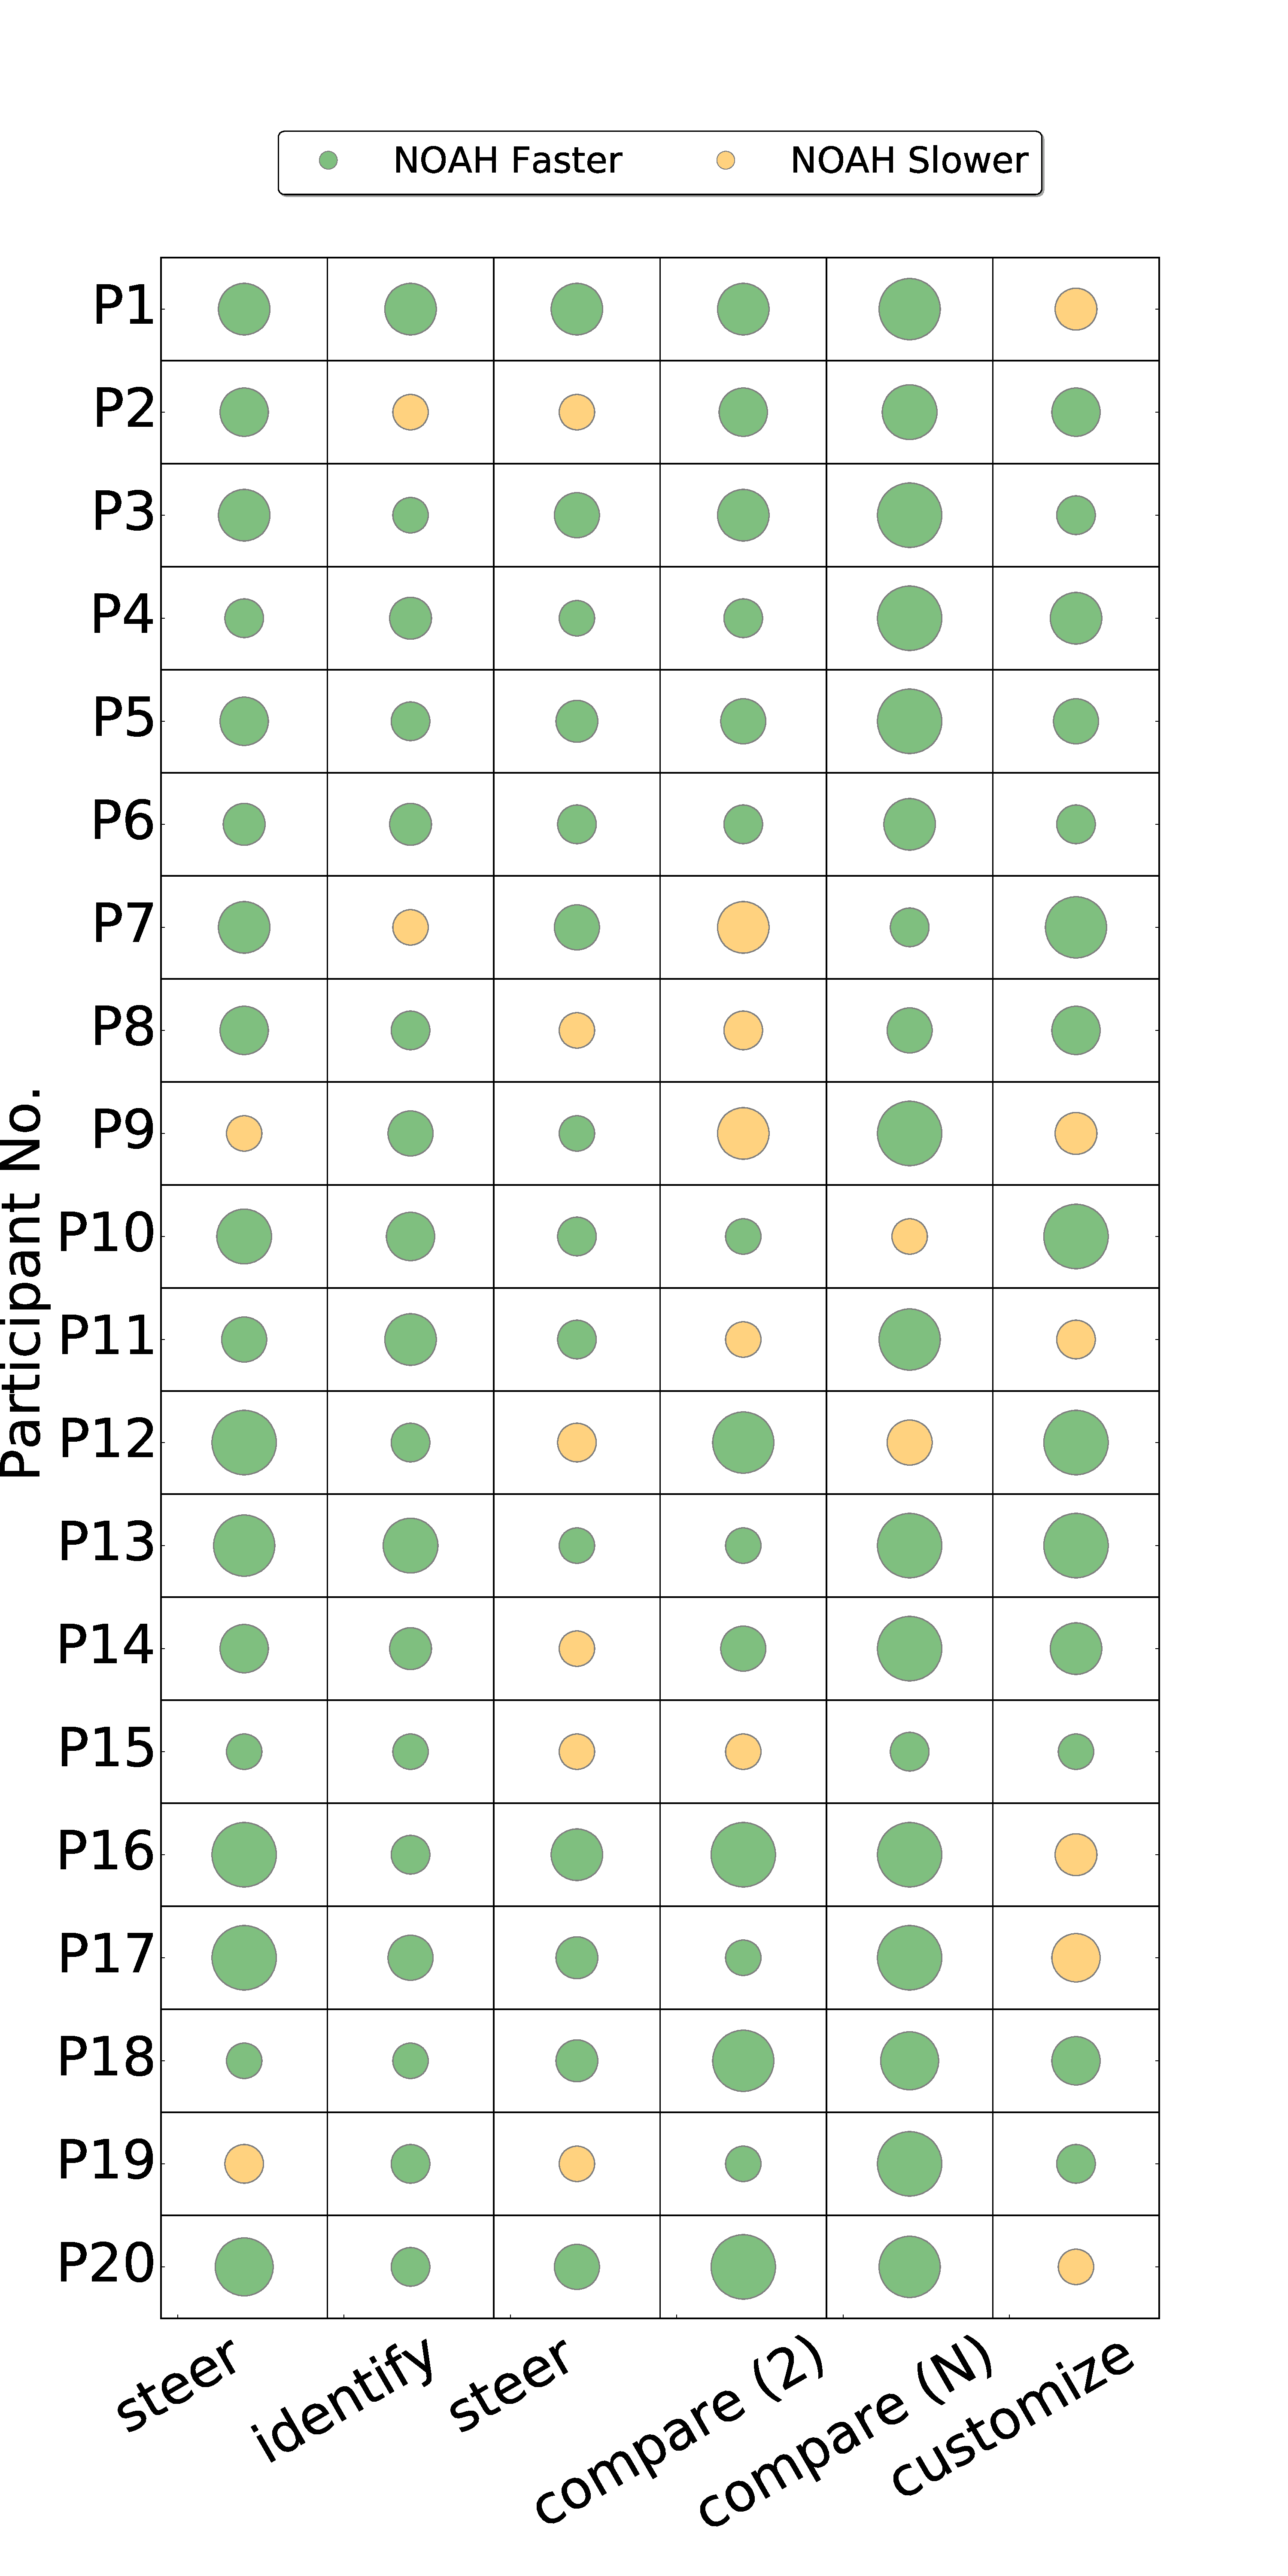
\includegraphics[trim=0 0 0 0,clip,width=\linewidth]{images/userinfo-ip.pdf}
\vspace{-20pt}
   \caption{Intra-participant submission time differences between \noah and Excel across the quiz tasks.}
\vspace{-15pt}
   \label{fig:ipdiff}
 \end{figure}
 
\subsection{Qualitative Observations}
\label{sec:interview_result}\label{sec:survey_result}
We now present a qualitative analysis of the participants' perceptions of both tools based on their interview responses.

\stitle{Data comprehension easier in \noah.} 
Without an overview, participants found it difficult to 
perform various tasks on Excel---\emph{Excel can get overwhelming 
if you have a lot of data in it and sometimes with that data 
finding things can be difficult ($P11$).} 
The binned representation of the data in \noah, 
on the other hand, helped users to comprehend 
the overall structure of the data better 
and prioritize the bin they want to visit next, enabling faster navigation. 
Out of 20 participants, 15 preferred \noah for tasks involving navigation. 
One participant ($P5$) commented: 
\emph{I think it was just a little bit easier to navigate 
and find where things were because you could already see what bins had what.} 
Another participant ($P1$) commented:  
\emph{I like \noah a lot better. It was a lot easier to look up different data 
and it was a lot quicker too}. 
Participants ($N=6$) additionally mentioned 
that they would prefer \noah over Excel when the dataset is large. 
One participant ($P2$) commented: 
\emph{I guess if I just had a large amount of data 
then I would prefer to use \noah because then you 
would be able to see all of it $\ldots$at once.} 
Finally, participants preferred the automatic data highlighting 
feature while performing the \emph{identify} task (16 out of 20). 
The colored cells focused their attention 
to relevant spreadsheet regions---\emph{It was a visual 
cue right there, made it very quick to count it up ($P17$).}
However, one participant ($P5$) mentioned the fact that 
some of the color choices would make \noah unusable 
for the colorblind population.

\toappendix{
\stitle{Overview-Spreadsheet Coordination.} Out of 20 participants, 16 participants preferred the automatic data highlighting feature of \noah while performing the \emph{identify} task. Moreover, the colored cells focused their attention to relevant regions within the spreadsheet---\emph{You didn't have to do any additional steps and it was a visual cue right there, made it very quick to count it up ($P17$).} However, one participant ($P5$) mentioned the fact that some of the color choices would make \noah unusable for the colorblind population.
}

\stitle{Scrolling and steering is cumbersome in Excel.} 
Participants found scrolling and steering in Excel 
to be cumbersome while issuing formulae 
and performing comparisons---\emph{The one thing 
with Excel is I always try to go to the bottom of the data 
and type in the formula, and with something really long like this, 
the scrolling is a little bit cumbersome ($P4$).} 
With \noah users can 
(a) avoid scrolling by using clicking or zooming operations, 
and (b) avoid steering by performing aggregate operations on the overview. 
One participant ($P3$) commented: 
\emph{And that creates convenience sort of because then you don't have to memorize anything and using the system becomes easier.} 
Another participant commented: \emph{With \noah, 
you don't have to highlight every number $\ldots$ 
versus Excel you actually have to select everything ($P12$).} 

\stitle{Fine-grained control is powerful but sometimes difficult to use.}
The bin customization feature enables users to 
personalize the overview based on their specific needs. 
One participant ($P16$) commented: 
\emph{I did like the fact that it lets you take a data sheet and, in some way, containerize the stuff you care and the stuff you don't care about.} 
14 out of 20 
participants found the bin customization feature to be useful. 
Participants preferred the feature to Excel’s filtering feature 
when working with numeric data---\emph{That was so much easier in \noah 
than it was in Excel to be able to specify the range that you wanted it to go in ($P17$).} However, six participants found the feature to be difficult 
to use when working with textual data and would have 
preferred a pivot table-like single level overview---\emph{I would have expected them to completely be split, 
and then I can merge them if I want to ($P13$).}

\stitle{Participants preferred \noah to Excel on all subjective user satisfaction metrics ({\em RQ4})} Figure~\ref{fig:survey} displays the subjective participant ratings 
for various satisfaction metrics using a diverging stacked bar chart. 
For a given metric, each white ellipse denotes the average rating 
given by the participants for the corresponding tool. 
We can see from the figure that participants preferred \noah to Excel 
for all metrics. 
Notably, participants found \noah to be easier to use 
compared to Excel, while being faster in execution. 
Even though the features offered by \noah were new to participants 
they found it fairly easy to learn. 
\toappendix{We further conducted a statistical significance test---the \emph{Wilcoxon Signed-rank} test---on the survey responses which showed that for all the metrics, the ratings significantly differed by the choice of the tool, \ie \noah or Excel. 
The distribution of the ratings for none of the criteria followed a normal distribution.}



\begin{figure}
    \centering
    %\vspace{-10pt}
    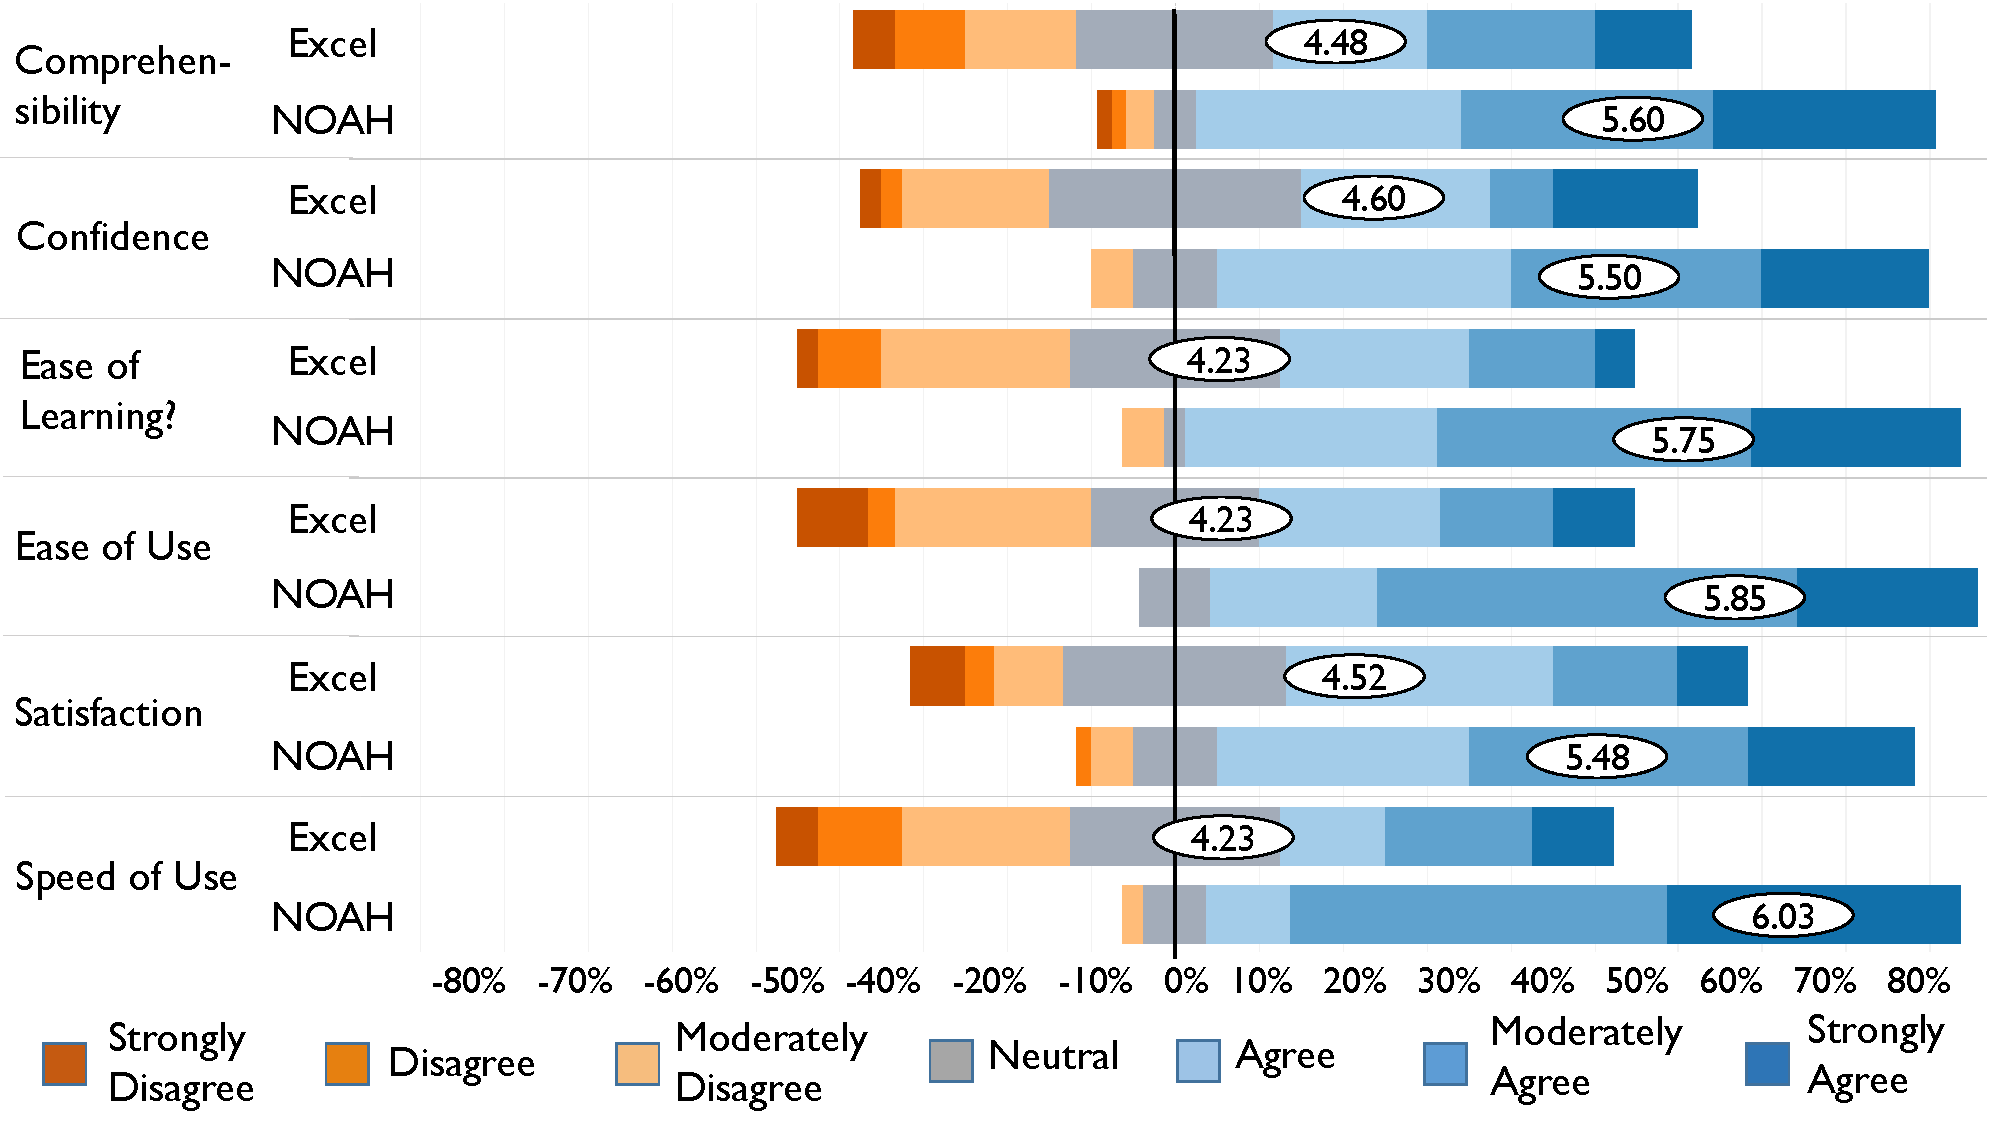
\includegraphics[trim=0 0 0 0,clip,width=\linewidth]{images/survey.pdf}
\vspace{-20pt}
   \caption{Participants found \noah to be easier to use compared to Excel while being faster in completing tasks involving navigation.}
\vspace{-15pt}
   \label{fig:survey}
 \end{figure} 

\toappendix{
\begin{table}[!htb]{\scriptsize}
\caption{Survey results. (*) indicates statistical significance. }
\label{tab:survey}
\centering
\begin{tabular}{|l|l|l|l|}
\hline
Metric &    \noah   &    Excel   & $p$ value \\ \hline
Ease of Learning &  $\mu = 5.75$, &    $\mu = 4.22$, & $\mathbf{1.49 \times 10^{-7}}$ (*) \\
& $\sigma = 1.02$ & $\sigma = 1.41$ & \\\hline
Speed of Use &    $\mu = 6.03$, & $\mu = 4.22$, & $\mathbf{1.68 \times 10^{-7}}$ (*)\\
& $\sigma = 0.99$ & $\sigma = 1.65$ & \\\hline  
Ease of Use    & $\mu = 5.88$, & $\mu = 4.33$, & $\mathbf{7.85 \times 10^{-6}}$ (*) \\
& $\sigma = 0.90$ & $\sigma = 1.71$ & \\\hline
Confidence    & $\mu = 5.50$, & $\mu = 4.60$, & $\mathbf{0.0096}$ (*)\\
& $\sigma = 1.79$ & $\sigma = 1.50$ & \\\hline  
Comprehensibility & $\mu = 5.60$, & $\mu = 4.48$, & $\mathbf{0.0006}$ (*)\\
& $\sigma = 1.27$ & $\sigma = 1.65$ & \\\hline
Satisfaction & $\mu = 5.48$, &    $\mu = 4.52$, & $\mathbf{0.0018}$ (*)\\
& $\sigma = 1.16$ & $\sigma = 1.49$ & \\\hline
\end{tabular}
\end{table}
}
\section{Discussion}
\label{sec:discuss}

In this section, we discuss the shortcomings of our user study, 
the limitations of \noah as a spreadsheet plug-in for navigation, 
and possible enhancements.

\subsection{Limitations}
We first discuss the limitations of \noah. 

\stitle{Limitations of Study Design.} Our evaluation compared a \noah-integrated spreadsheet with a traditional spreadsheet. However, it is certainly possible to evaluate intermediate versions of \noah that isolate the effects of the zoomable overview (visual clarity vs.~visual continuity), display layout (screen space trade-off), and 
contextual presentation of data (raw text vs.~chart representation of aggregate columns). Moreover, our participant pool demographics may not match the demographics of the general audience intended for this tool. 

\stitle{Unfamiliarity with \noah.} Several interactions on \noah 
are quite different from typical spreadsheet interactions, \eg zooming, bin customization. 
This unfamiliarity led to some participants ($N=5$ out of 20) 
preferring Excel over \noah. \toappendix{One participant ($P11$) commented: \emph{Since I'm not used to spreadsheet data being presented that way, it took a little bit of getting used to.}} Participants found some of the terminologies 
used in the interface---\eg explore, bin---to be quite 
unfamiliar ($N=14$)  for an Excel audience. 
Moreover, two participants didn’t understand how the bins were constructed. 
These issues can be addressed by using more relatable terminologies and proper documentation. 
Two participants found the aggregation operations 
applied on the bins to be opaque compared to Excel 
where a user can directly manipulate the formula\toappendix{---\emph{I like the way that in Excel I can go look at my formula again if I wanted to make sure I'm doing everything I wanted to do correct ($P6$)}}. 
In subsequent versions of \noah, we can further 
display the appropriate formula for each bin as users hover 
over the corresponding cell on the aggregate column. 
Moreover, participants ($N=5$) noted the fact that \noah currently 
does not support user defined formulae.

\stitle{Binning Mechanism.} \saj{A number of participants ($N=6$)
did not prefer the current binning mechanism for categorical data. 
As explained in Section~\ref{sec:design},
the purpose of such binning
was to reduce visual discontinuity.
The outcomes of the \cmpB tasks in Section~\ref{sec:results}
further justifies this choice 
as participants ended up
making more mistakes
when the overview displayed all the unique bins.
However, the experience 
surrounding the construction
of the overview
can be further improved.
Currently, the bins of the overview
can be customized
only after the overview is constructed.
Providing the users
the capability to
select the representation
(similar to bin customization)
of the overview could have addressed this issue.
Understanding the impact of these
representation choices for the overview
can be an interesting future research.}

\subsection{Future Work}
We now discuss the to further enhance the capabilities of \noah. 

\stitle{Beyond Tabular Data.} \noah operates only on tabular data. 
However, spreadsheets can be semi-structured---formulae 
and text can be interspersed with tabular data. 
We can extend \noah to act as a map highlighting heterogeneous regions on such complex spreadsheets which users can utilize to navigate the spreadsheet. 
We can leverage existing work on spreadsheet table detection~\cite{tablesense}, 
and property identification~\cite{chen2017spreadsheet} 
to construct the map.  

\stitle{Scope of Overview-Spreadsheet Coordination.} \saj{can we generalize this to an unified framework.}
Spreadsheet users may perform various edit operations, 
\eg updating values, adding/deleting rows/columns. 
However, \noah currently assumes the data to be read-only. 
In our next version, we can add support for 
propagating the spreadsheet updates to the overview. 
Moreover, the charts displayed in an \emph{aggregate column} are non-interactive, 
\ie users cannot interact with the charts to visually look up relevant or 
interesting data points within the spreadsheet. 
In the future, we plan to extend \noah to support visual querying 
through the charts in an aggregate column.

\stitle{From Perceptual to Interactive Scalability.} 
The current version of \noah addresses the perceptual 
scalability challenges while navigating 
Excel-scale (one million rows) data. 
As modern spreadsheets continue to support 
even more large scale data---{\scshape DataSpread}~\cite{datamodels} 
supports one billion rows---the interactions proposed in this paper may violate the interactive response time bound of 500 ms~\cite{liu2014effects}. This opens the door to a new set of research challenges that may range from approximate query processing to progressive data analytics.

\stitle{Other Enhancements.} \noah currently constructs the overview on a single attribute. We can add support for multi-attribute navigation (\eg explore the Airbnb data by city and neighborhood), and multi-level navigation (\eg explore the neighborhoods after zooming into a specific city in the Airbnb data). \toappendix{Moreover, as shown in Section Table~\ref{tab:scope}, \noah does not allow users to add annotations, \eg visual cues, texts, to the overview. These operations can be implemented in the future as feature extensions.} Furthermore, bin customization currently supports changing the bin boundaries only while maintaining the current order. Supporting user defined ordering to allow arbitrary reshuffling of the bins can be another enhancement.\toappendix{ However, such modification will require a redesign of the histogram based data structure since the ordering property will not hold anymore.} Finally, a complete characterization of the spreadsheet operations that can be supported by \noah is another open question, \eg other operations that involve working with subsets of spreadsheet data, \eg sorting, filtering, copy-pasting.

\section{Conclusions}
\label{sec:conclusion}
We presented \noah, an in-situ navigation interface, designed as a spreadsheet plugin.
Using \noah, users can get a bird’s eye view of the data, with the ability to scroll or seek
additional details on demand, using a multi-granularity overview, as well as
aggregate columns that eliminate cumbersome steering operations.
We conducted a user study that demonstrated that participants found \noah to be much more easy to use compared to Excel for navigating large spreadsheet datasets. Across different navigation tasks, participants were able to attain 
higher accuracy when using \noah compared to
Excel while being twice as fast. 
\noah represents our 
first step towards making spreadsheets more effective 
on large datasets that are increasingly the norm.